\documentclass{beamer}
\usepackage{geometry}
\usepackage{amssymb, amsmath, amsfonts, graphicx}
\graphicspath{ {/}{images/}}

\DeclareMathOperator{\lcm}{lcm}

\title{Elliptic Curves}
\author{Jake Fisher and Davis Lister}
\date{May 1, 2018}
\begin{document}	
	\begin{frame}
		\titlepage
	\end{frame}
	
		\begin{frame}{Group Law for Elliptic Curves}
		\begin{itemize}
			\item Elliptic Curves are a group under the $+$ operation with the set $\lbrace K \times K: y^2=x^3+ax+b \rbrace \cup \lbrace \mathcal{O} \rbrace$ where $\mathcal{O}$ is the point at infinity and $K$ is a field. We notate the set of elliptic curves over a field $K$, $(E(K))$.
			\item Let us define the discriminant $\Delta = -16(4a^3+27b^2)$. If $\Delta = 0$ the group law does not hold.
			\item The $+$ operation is defined geometrically on two points $(x_1,y_1)$ and $(x_2,y_2)$ thus: draw the secant line and find the third point where it intersects the curve $(x',y')$, which can include $\mathcal{O}$, finally find $(x',-y')$, the resulting point.
			\item Under the $+$ operation $\mathcal{O}$ is the identity and $(x,y)^{-1}=(x,-y)$.
			\item All computations are done over the set $\mathbb{Z}/n\mathbb{Z}$ in cryptographic and integer factorization applications.
		\end{itemize}
	\end{frame}
	
		\begin{frame}{More on the Discriminant}
		\begin{itemize}
			\item The condition we impose on the discriminant is the is motivated by the need to have a tangent line be well defined at all points on the curve $S\in(E(K))$. If the tangent line is not defined at a point $P_0=(x_0,y_0)$, then $S$ is singular.
			\item If S is singular, then $P_0+P_0$ is not well-defined, which breaks the group law.
			\item Geometrically, a singularity is a cusp or self-intersection.
			\newline 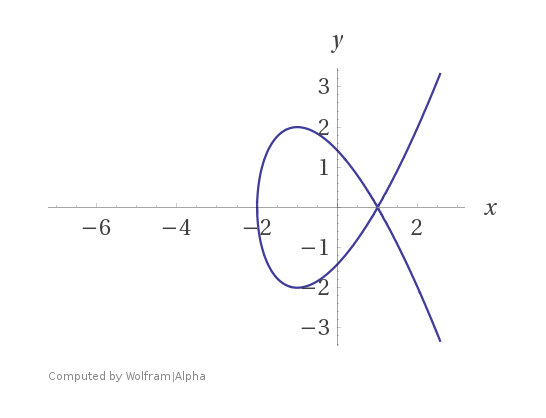
\includegraphics[scale=.3]{SingularCurve.png}
		\end{itemize}
	\end{frame}
	
	\begin{frame}{Definition of $B$-power smooth}
		\begin{itemize}
			\item Let $B$ be a positive integer. The prime factorization of an integer $n=\prod p_{i}^{e_{i}}$. If $\forall i$ $p_{i}^{e_{i}} \leq B$, $n$ is $B$-power smooth.
			\item For instance, $60$ is $5$-power smooth but $150$ is $25$-power smooth.
		\end{itemize}
	\end{frame}
	
	\begin{frame}{Pollard's p-1 Factoization}
		\begin{itemize}
			\item We wish to find a nontrivial factor of a large positive integer $N$ using the Pollard p-1 method.
			\item Let us choose a positive integer $B$. Suppose that there is a prime factor $p$ of $N$ such that $p-1$ is $B$-power smooth.
			\item Let us choose $a > 1$ such that p does not divide a. Often we will choose $a=2$ for convenience.
			\item By Fermat's Little Theorem $a^{p-1} \equiv 1 \mod p$.
			\item Let $m = \lcm (1,2,3,\dotso,B)$. Since $p-1$ is $B$-power smooth, $p-1 \mid m \Longrightarrow p \mid \gcd (a^m-1,N) > 1$.
			\item If $\gcd (a^m-1,N) < N$, then $\gcd (a^m-1,N)$ is a nontrivial factor of N.
			\item The algorithm becomes more transparent if we consider $m=k(p-1)$, where $k\in\mathbb{Z}$.
		\end{itemize}
	\end{frame}
	
	\begin{frame}{Factoring Magic!}
		\begin{itemize}
			\item An example of integer factorization using Pollard's p-1 method.
			\item Let $N=5917$ and let $B=5$. $m=\lcm (1,2,3,4,5)=60$.
			\item Note that $2^{60}-1=3416 \mod 5917$, and $\gcd (2^{60}-1, 5917)=\gcd (3416, 5917)=61$.
			\item 61 is a factor of 5917!
			\item But if $p-1$ and $q-1$ (where $pq=N$) are not $B$-power smooth, Pollard p-1 does not work.
			\item The issue is that $(\mathbb{Z}/p\mathbb{Z})^*$ has order p-1.
			\item Additionally, if $p-1$ is the product of many small primes, then the algorithm will return $N$.
		\end{itemize}
	\end{frame}
	
	\begin{frame}{Lenstra's Elliptic Curve Factorization}
		\begin{itemize}
			\item 
		\end{itemize}
	\end{frame}
\end{document}